\section{Appendix}
\label{appendix}

\subsection{Choosing model parameters}

\begin{figure}[!h]
    \centering
    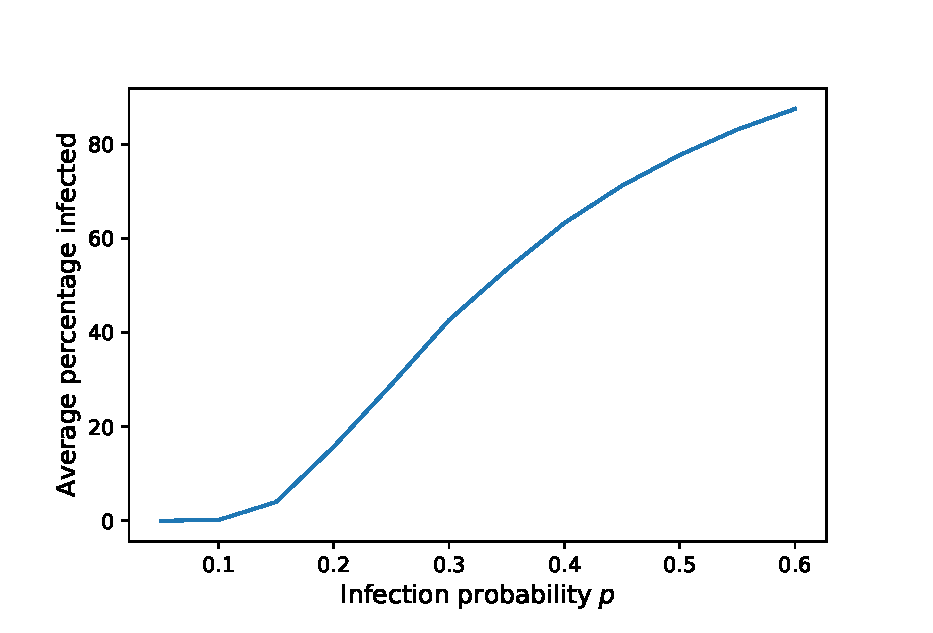
\includegraphics[scale = 0.55]{Figuresnew/PA_attackrates.eps}
    \caption{Preferential: p vs avg. percent infected.)}
    \label{fig:PA_ar}
\end{figure}

\begin{figure}[!h]
    \centering
    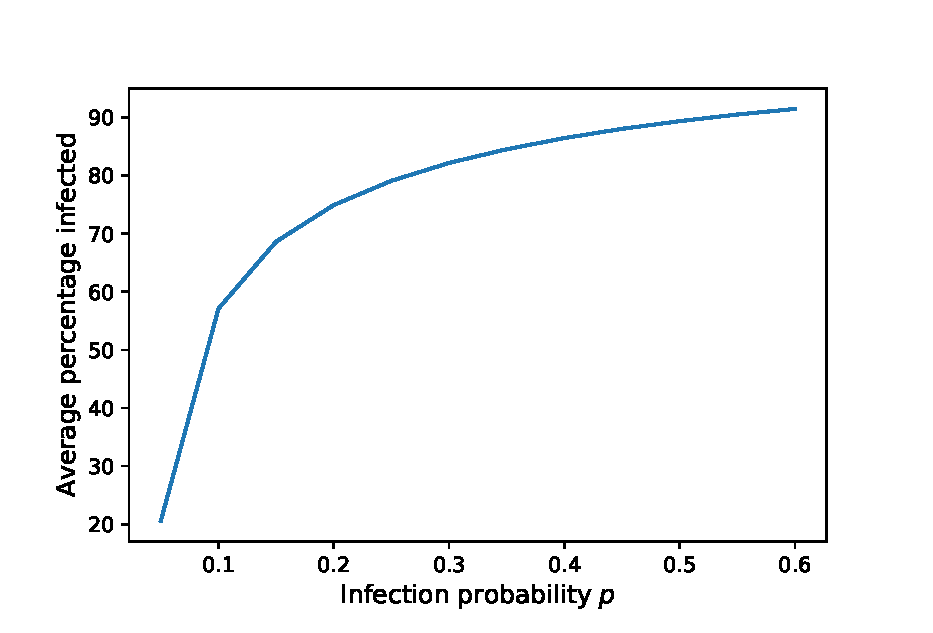
\includegraphics[scale = 0.55]{Figuresnew/montgo_attackrates.eps}
    \caption{Montgomery: p vs avg. percent infected.}
    \label{fig:montgo_ar}
\end{figure}



\begin{figure}[!h]
    \centering
    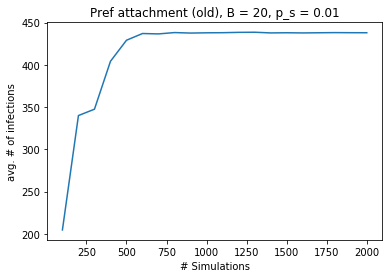
\includegraphics[scale = 0.6]{Figuresnew/simulations.png}
    \caption{Simulation vs average infected (Preferential Attachment PA1)}
    \label{fig:pa_simvsavg}
\end{figure}

\begin{figure}[!h]
    \centering
    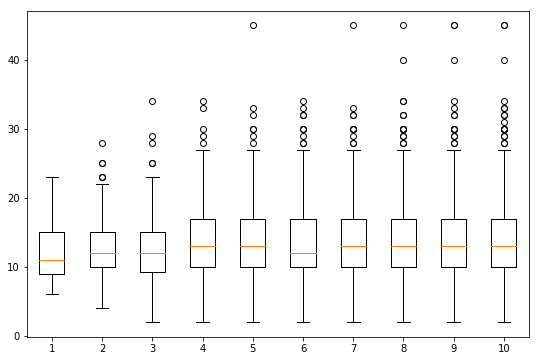
\includegraphics[scale = 0.42]{Figuresnew/boxplotPA2.png}
    \caption{Number of infections over the $M$ samples (y-axis) vs $M/50$, i.e., the number of samples (in 50s) on the x-axis
for the Preferential Attachment (PA2) network}
    \label{fig:pa2_bloxplot2}
\end{figure}

\subsection{Parameters used to generate random networks}
We use Networkx to generate the random graphs PA1, PA2, and SW.

Preferential1 (PA1): $barabasi\_albert\_graph(n=1000, m=2, seed=None)$\\

Preferential (PA2):  $barabasi\_albert\_graph(n=100000, m=2, seed=None)$\\

Small World (SW): $navigable\_small\_world\_graph(n=50, p=1, q=5, r=2, dim=2, seed=None)$\\

\subsection{Infection probability Used}
Small World (SW): $p = 0.1$ \\
Preferential1 (PA1): $p = 0.3$ \\
Preferential2 (PA2): $p = 0.125$ \\
Portland : $p = 0.03$ \\
Montgomery : $p = 0.045$ \\

\noindent
Budgets used in experiments where it is not specified is $B = 50$.

